\documentclass[../main.tex]{subfiles}

\begin{document}

\section{User Management}
\label{section:lauxus:user_mgnmt}

\par Users within LAUXUS are identified by a unique random UUID and are authenticated with an asymmetric key pair. This key can be generated by LAUXUS if the user requested it. Asymmetric encryption enables secure authentication to the filesystem (e.g: like SSH authentication), as we will see later. We used Elliptic-curve cryptography keys as these primitives are, by default, implemented within SGX Enclave Package.


\subsection{User registration/deletion}
\label{section:lauxus:user_registration/deletion}

\par Users can only be registered by the administrator (cfr. Section \ref{section:lauxus:login}). Users are added to the list of authorised user simply by adding their public key and assigning them a UUID. The administrator is responsible of verify the authenticity of the public key he received. The transmission of this public key is an orthogonal problem that will not be discussed here.
\par The user UUID will be used within the entitlement in Section \ref{section:lauxus:user_entitlement}. Afterwards, users can login by using their UUID and their private key. We used random UUID to identity user instead of their "username" (like other classical login procedure). This chose is motivated thanks to its simplicity and making a more elaborated user management is not really in the scope of our work. Although, it would be interesting as an improvement to the project.
\par Removing a user is even more straightforward, the administrator only needs to remove the user public key from the database.


\subsection{Login protocol}
\label{section:lauxus:login}

\begin{figure}[ht]
    \centering
    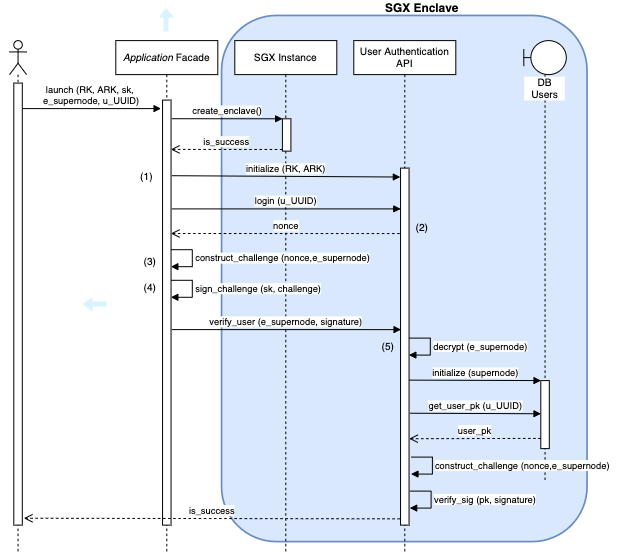
\includegraphics[width=\textwidth]{images/lauxus/user_login}
    
    \caption{Login sequence diagram}
    \label{figure:lauxus:login}
\end{figure}
\par As the sequence diagram in Figure \ref{figure:lauxus:login} is enough to understand the user login process, we will only give some complementary details (according to the numbers on the Figure):
\begin{itemize}
    \item[1)] \textit{RK} and \textit{ARK} stands for "Root Key" and "Audit Root Key".
    \item[2)] The \textit{nonce} is randomly generated inside the Enclave and is big enough to avoid duplicates.
    \item[3)] The challenge is constructed by concatenating the generated nonce and the encrypted content of the supernode. This allows to binds the nonce to the current state of the supernode. This avoids the supernode to be changed during the login procedure (in the case the user is revoked between the start of the login process and the end).
    \item[4)] The signature and verification of the challenge is done thanks to the asymmetric property of ECC.
    \item[5)] The supernode is decrypted following the protocol explained in the Metadata decryption Section \ref{section:lauxus:metadata_encryption}.
\end{itemize}
\par In a nutshell, the login process allows to:
\begin{itemize}
    \item \textbf{Verify the identity of the user} thanks to the signature provided and the public key stored inside the supernode.
    \item \textbf{The user is authorised to access the filesystem} thanks to the presence of his public key inside the supernode.
    \item \textbf{The supernode hasn't been tampered with} thanks to the metadata encryption protocol.
    \item \textbf{The supernode is linked to the given root-key} thanks to the metadata encryption protocol.
\end{itemize}


\subsection{User entitlement}
\label{section:lauxus:user_entitlement}

\par As we have discussed above, user are identified by using UUID. These UUID are used for the user entitlement. Each file and directory in the filesystem has an entitlement database stating which UUID can access the given resource. The entitlement is composed of 4 flags: ownership permission, read permission, write permissions and execution permission (1 bit per flag, like UNIX RWX permission). Only the administrator and the owner of a file can assign the entitlement to this specific file (a user is the owner of a file if the ownership flag is set to 1).
\par Note that these UUID are not related to the Unix user ID. In fact, LAUXUS never rely on these Unix user ID. The only exception is when providing the owner of a file. We decided that the user who launched LAUXUS will be the owner of all the files. For security reason, only the owner of the file can access it. Other UNIX users (users in the same group or others) permissions are always set to 0. In this way, no-one except the launcher of the application (the user we authenticated) can access the filesystem.


\end{document}